% v2-acmsmall-sample.tex, dated March 6 2012
% This is a sample file for ACM small trim journals
%
% Compilation using 'acmsmall.cls' - version 1.3 (March 2012), Aptara Inc.
% (c) 2010 Association for Computing Machinery (ACM)
%
% Questions/Suggestions/Feedback should be addressed to => "acmtexsupport@aptaracorp.com".
% Users can also go through the FAQs available on the journal's submission webpage.
%
% Steps to compile: latex, bibtex, latex latex
%
% For tracking purposes => this is v1.3 - March 2012

\documentclass[prodmode,acmtecs]{acmsmall} % Aptara syntax
\usepackage{float}

\usepackage{natbib}
\usepackage{hyperref}
\usepackage{amssymb}
\usepackage{subcaption}
\usepackage{enumitem}
\usepackage{tabularx,ragged2e,booktabs}
\usepackage{rotating}
\usepackage{tikz}
\usetikzlibrary{calc,positioning,backgrounds,arrows.meta}
\usepackage{forest}
\usepackage{multirow}
\usepackage{array}
\usepackage{pifont}
\usepackage[english]{babel}
\newcommand*\rot{\rotatebox{90}}
\newcommand*\OK{\ding{51}}

\newcolumntype{P}{>{\raggedright\arraybackslash}p}

%\usepackage{amsthm}
\usepackage{mathtools}
\newtheorem{mydef}{Definition}
\newcommand{\mydefautorefname}{Definition}

\addto\extrasenglish{%
  \renewcommand{\sectionautorefname}{Section}%
  \renewcommand{\subsectionautorefname}{Section}%
  \renewcommand{\subsubsectionautorefname}{Section}%
  \renewcommand{\algorithmautorefname}{Algorithm}
}

% Package to generate and customize Algorithm as per ACM style
\usepackage[ruled]{algorithm2e}
\renewcommand{\algorithmcfname}{ALGORITHM}
\SetAlFnt{\small}
\SetAlCapFnt{\small}
\SetAlCapNameFnt{\small}
\SetAlCapHSkip{0pt}
\IncMargin{-\parindent}


% Document starts
\begin{document}

% Page heads
\markboth{}{Comparison of Evaluation Protocols for Sequential Recommender Systems }

% Title portion
\title{Comparison of Evaluation Protocols for\\ Sequential Recommender Systems }
\author{
MS. UMBERTO DI FABRIZIO
\affil{Politecnico di Milano}
Tutor: Ph.D MASSIMO QUADRANA
\affil{Politecnico di Milano}
Prof. PAOLO CREMONESI
\affil{Politecnico di Milano}
}
\begin{abstract}
Recommender Systems are used to predict the user appreciation for some future items. One trend is to exploit the recent history of a user actions in order to enhance the performances of the recommender. Such sequential recommender systems (SRS) can be evaluated using different protocols, namely set or sequential. To this day, there has been no evaluation of the result obtained using one protocol over the other. In this work the protocols are compared with respect to the ranking among six classes of SRS using both precision and recall metrics, moreover the sensitivity of each protocol in comparing the recommenders is discussed. The results show that, even though there is almost no difference in the results produced by the two protocols, the set one may be the favorable choice given his highest sensitivity and faster run time.  
\end{abstract}
 
\keywords{Sequential Recommendation, Evaluation protocols}

\maketitle


%%%%%%%%%%%%%%%%%%%%%%%%%%%%%%%%%%%%%%%%%%%%%%%%%%%%%%%%%%%%%%%%%%%%%%%%%%%%%%%%
\begin{abstract}
	In this work several Sequential Recommender Systems (SRS) are evaluated accordingly to two evaluation procedures.
\end{abstract}


%%%%%%%%%%%%%%%%%%%%%%%%%%%%%%%%%%%%%%%%%%%%%%%%%%%%%%%%%%%%%%%%%%%%%%%%%%%%%%%%
\section{INTRODUCTION}
%che cos'e SRS
Recommender Systems are used to predict the user appreciation for some future items. Traditionally RSs attempt to make such predictions based on item-similarity or user-similarity as well as hybrid techniques, yet most often the behavior of a user is strictly related to the last actions performed e.g. last songs listened, last items purchased, last apps opened. For this reason it seems reasonable to exploit the user profile/context i.e. the last actions performed by an user, in order to make more reliable and accurate predictions. In the literature there are several systems that try to exploit the recent history of an user's actions, namely Sequential Recommender Systems (SRS).\\There are several approaches to build a SRS (which will be discussed in the next section) as well as several protocols to assess the performances of such items and it is of undeniable importance the assessment of different SRS accordingly to the same protocol.
\\
The objective of this work is to implement several classes of sequential recommender systems in order to compare their performance adopting two evaluation protocols: set and sequential. In the next sections the extent to which the two protocols may produce different results when assessing multiple recommenders is analyzed.
\section{CLASSES OF SEQUENTIAL RECOMMENDER SYSTEMS}
The classes of SRS that are used in this work are taken from the state-of-the-art SRS:
\begin{enumerate}
	\item \textbf{Popularity based} recommender is non-personalized and doesn't exploit the recent history of a user, yet it has been included for comparison purposes. The popularity recommender always predicts the top N most popular items.
	\item \textbf{Frequent Pattern Mining}\cite{mobasher02sequential} recommenders incorporate history in the system by leveraging on the ability to mine frequent sequences in the dataset and in so doing they can learn which sequences of items are more frequent, thus they can recommend the most probable next-item. The algorithm implemented adapts the SPMF library\cite{fournier2016spmf} and a prefix tree structure to keep sequences in memory. Once a pattern in the prefix tree is matched the children of the last node in the matched path are recommended as next items.
	\item \textbf{Markov Chain} recommenders \cite{shani05mdp} build a state graph where each state is a sequence of length k and k is the order of the markov model. In the simplest approach there is an edge between two states if the dataset has at least an occurrence of length k+1 made by concatenating the sequence in the first state with the last item of the next state. This definition is augment as proposed in \cite{shani05mdp} by applying skipping, clustering and model mixing. Although a markov model represents a clear method to exploit the sequence's history, it is computationally expensive in terms of both memory and running time, for this reason it has been constrained to a first order model. 
	\item \textbf{Prod2Vec} recommenders\cite{grbovic15prod2vec} are based on the theory of n-grams developed by the NLP community which takes into account the context in which a word is found and creates a distributed representation of that word. Word2Vec models have been used virtually in all types of applications\cite{any2vec}, in the case of recommender systems items (=words) are projected into a vector space by taking into account their context (=the k items before and after the one considered in the sequence). Similarity among items is calculated by applying the cosine similarity among their distributed representations. In this case the gensim\cite{rehurek2010software} library has been adapted to produce recommendations.
	\item \textbf{Supervised} recommenders try to model the historical data in such a way that classical atemporal machine learning algorithms can be used to make recommendations. In this work the \textit{data expansion} approach suggested in \cite{zidmars01temporal} has been used, together with a decision tree in order to obtain the final SRS.
	\item \textbf{Factorizing Personalized Markov Chains} represent a hybrid approach exploiting both the power of Markov Chains and Factorization models which have been extensively and successfully used in the literature of recommender system. This class of SRS has been built based on the paper\cite{rendle10FPMC} and by adapting the code at \cite{fpmcLib}.
\end{enumerate}
	The result of this work is a flexible library\cite{srsLib} which implements each of the recommender through a common interface and can be called from the command line by adding the optional configuration parameters.

\section{EXPERIMENT SET UP}
The dataset is composed of 10k unique items, 380k sessions and 28k users, collected from the LastFM website. In order to make this work feasible the number of unique items among the sequences has been reduced to 500, which has been chosen since the dataset size is manageable but the recommendation task is not trivial.
For each of the recommenders described in the previous section the two protocols of evaluation are executed for $k \in [1,5,10]$ where $k$ is the number of items in the user profile accordingly to the first-k approach: for each sequence only the first k elements are used to recommend the future elements. In the case of set evaluation the prediction list is compared with the ground-truth whilst for the sequence evaluation the first k element are used to make the first recommendation which is evaluated only w.r.t. the first element of the ground-truth,then the user profile length is increased by one and the items are recommended again, this process goes on until the ground-truth has length 0. In this way it is also useful to understand for which values of k the recommendations are more accurate.
Table~\ref{data} summarizes the statistics for the datasets adopted for each value of $k$.
For each recommender precision and recall are evaluated on a test set obtained by a random holdout split procedure 80/20, and the metrics are averaged on 5 runs.\\ The parameters used to run each recommender have been set by empirical evaluation by exploring the state space of the parameter, yet it is worth to notice that the scale of the metrics didn't vary significantly, appendix A provides the parameters choice.

\begin{table}[]
	\centering
	\caption{Dataset statistics}
	\label{data}
	\begin{tabular}{|c|c|c|c|}
		\hline
		\textbf{k} & \textbf{Train Size} & \textbf{Test Size} & \textbf{Average sequence length} \\ \hline
		1          & 102193              & 25549              & 4.65                             \\ \hline
		5          & 23973               & 5994               & 10.30                            \\ \hline
		10         & 6947                & 1737               & 17.34                            \\ \hline
	\end{tabular}
\end{table}

\section{RESULTS}
In this section the result of the comparison of the two protocols are presented and discussed.\\
For each $k$ (i.e. length of user profile) precision and recall are the metrics adopted to evaluate the performances of the recommenders.  
%grafo seq vs set, sia presicion che recall
Figures~\ref{img:precision_k_1}~\ref{img:precision_k_5}~\ref{img:precision_k_10} show the results for the precision metric for the considered values of $k$. In the graphs the x-axis represents the result for the set evaluation while the y-axis the result of the sequential evaluation. The decision to adopt such a visualization technique is twofold: firstly the more a classifier is far from the diagonal the more its performances vary between the two protocols, secondly it is quick to realize the effect of the different evaluation protocols in-fact any recommender that appears in the bottom right or the upper left has very different metric scores between the two protocols. By analyzing the figures it is evident that the set evaluation usually leads to higher scores for precision yet recall has the same magnitude for the two protocols, more importantly if the recommenders can be aligned in  a monotonic increasing order it means that the two protocols provide the same ranking when ordering the recommenders.
\begin{figure}[H]
	\centering			
	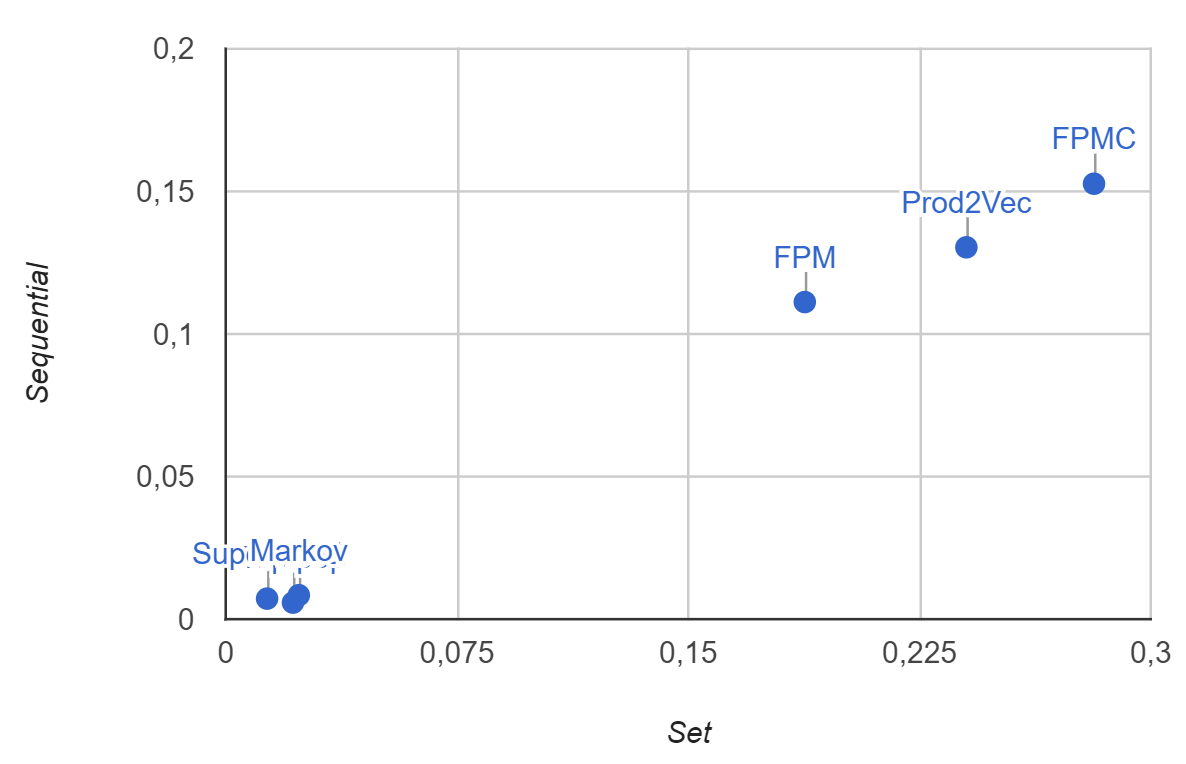
\includegraphics[width=0.8\textwidth]{img/precision_k_1.png}
	\caption{Precision scores for the set evaluation and the sequential evaluation, with $k=1$.}
	\label{img:precision_k_1}
\end{figure}
\begin{figure}[H]
	\centering			
	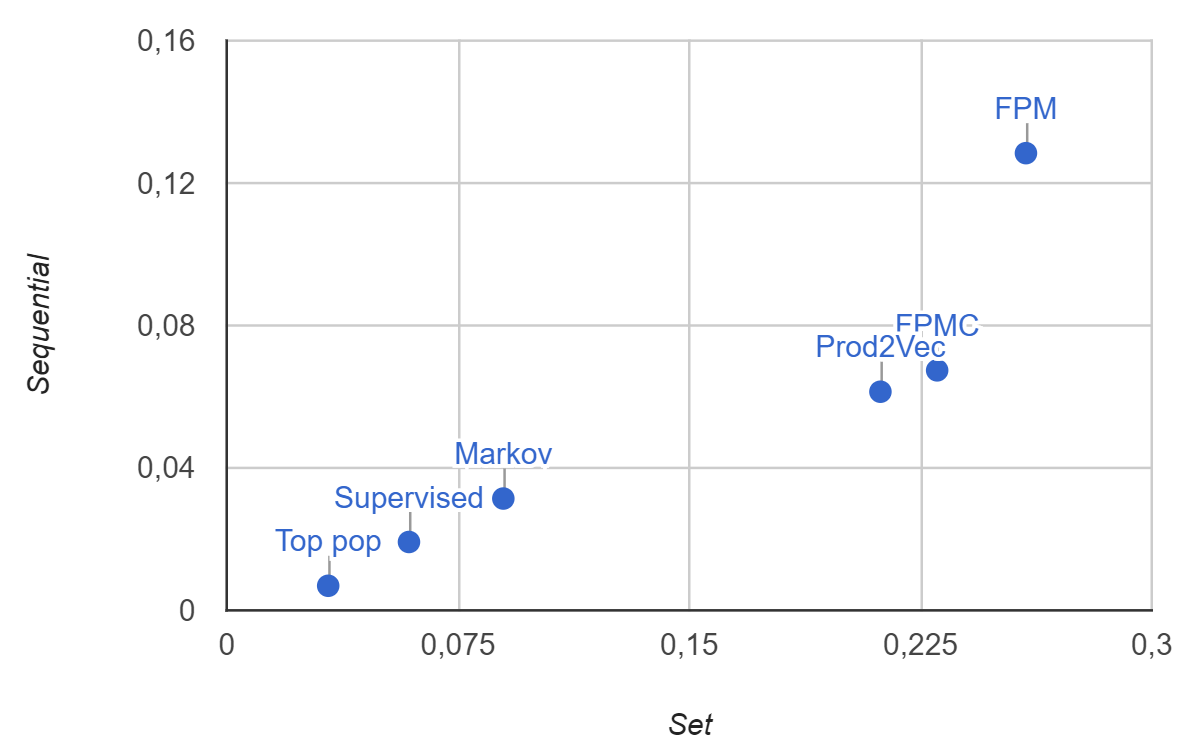
\includegraphics[width=0.8\textwidth]{img/precision_k_5.png}
	\caption{Precision scores for the set evaluation and the sequential evaluation, with $k=5$.}
	\label{img:precision_k_5}
\end{figure}
\begin{figure}[H]
	\centering			
	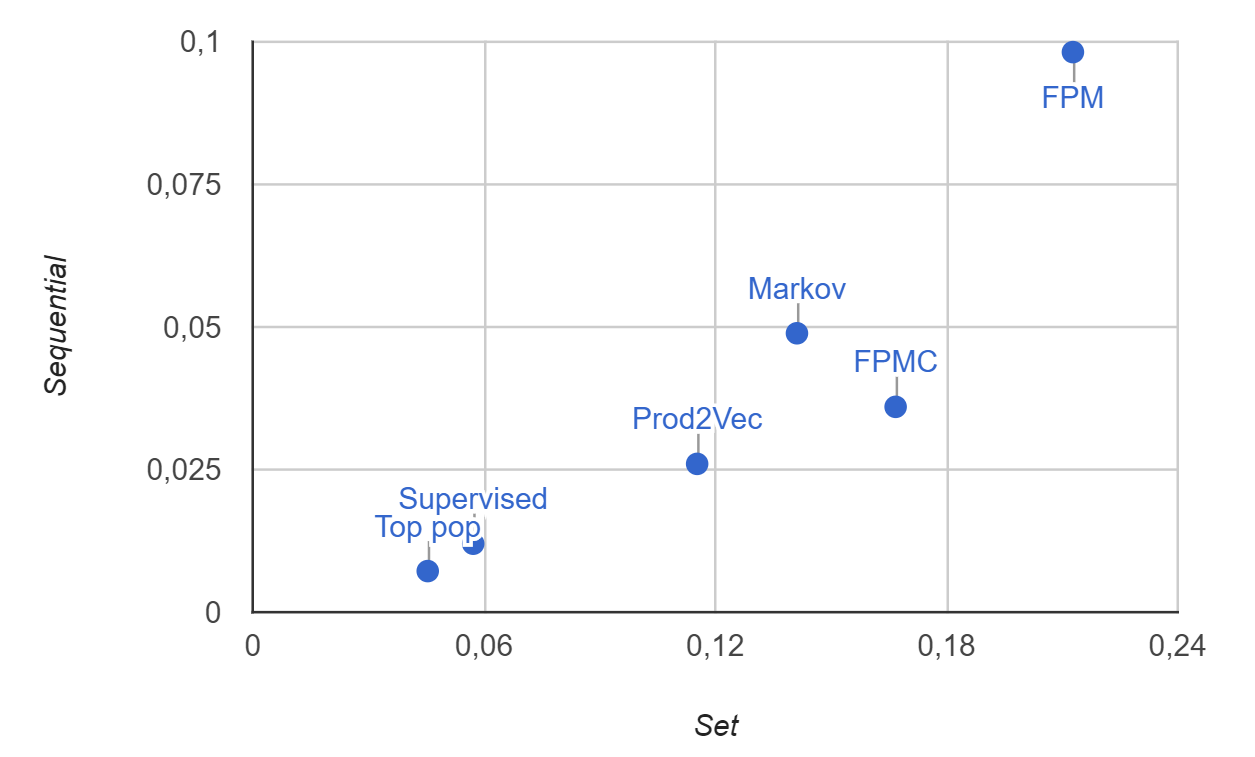
\includegraphics[width=0.8\textwidth]{img/precision_k_10.png}
	\caption{Precision scores for the set evaluation and the sequential evaluation, with $k=10$.}
	\label{img:precision_k_10}
\end{figure}

Since the interest is to verify the correct order of the ranking of the recommenders for both the evaluation protocols, the following measure has been adopted in order to evaluate the difference of the rankings produced by the evaluation protocols :
\[ r = \frac{\frac{1}{L} \sum_{i}(\frac{1}{d_i + 1}) - \frac{1}{L}} {1-\frac{1}{L}} \]
where $L$ is the number of recommenders and $d_i$ is the distance in terms of positions in the rankings between the two evaluation protocols, $r=1$ when there is perfect agreement in the rankings, $0$ when there's total disagreement. It is possible to see that for all the scores of precision~\ref{img:precision_k_1}~\ref{img:precision_k_5}~\ref{img:precision_k_10} and recall~\ref{img:recall_k_1}~\ref{img:recall_k_5}~\ref{img:recall_k_10} $r=1$ except for fig~\ref{img:precision_k_10} where $r=0.8$ because the Markov model is better than FPMC for the sequential evaluation but worst for the set evaluation.\\
Anyway comparing the rankings is not the only interest, infact it is also worth to compare the sensitivity of the two protocols, in other words one evaluation protocol may differentiate between recommenders much more that the other, for instance in fig~\ref{img:precision_k_5} the difference of precision among FPM and FPMC is $0.02$ for the set evaluation while $0.06$ for the sequential protocol.\\ It is important to evaluate the sensitivity of the two protocol because even though they may give the same ranking, one protocol may produce a much larger gap between two models than the other and this may cause misleading conclusions.\\
It is possible to capture the sensitivity given two recommenders $i,j$, by computing the absolute difference in the metric between $i,j$ using one protocol and subtracting the absolute difference of the metric between $i,j$ using the other protocol. In so doing if the metric score of the set evaluation among two recommenders differs of $0.02$ and the same metric using the sequence evaluation differs of $0.06$ it is possible to say that the sequential evaluation is more sensitive. This idea can be extended by adding up the sensitivity value among two recommenders for each pair of recommenders in the evaluation, leading to the formula:

\[sensitivity = \frac{\sum_{i,j} |set_i - set_j| - |sequential_i-sequential_j|}{2} \]
where $set_x$ is the metric score for recommender $x$ calculated using the set protocol whilst $sequential_x$ is the score calculated with the sequential protocol.
%division by two because the same score is calculate for i,j and j,i
Notice that the sensitivity value does not say anything about the ranking among the recommenders but addresses the magnitude of difference among them w.r.t. the metric used. Using together the $r$ value and $sensitivity$ score it is possible to say a) whether the two evaluation protocols produce the same ranking among the recommenders b) the scale of difference in the metric score among them.

\begin{figure}[H]
	\centering			
	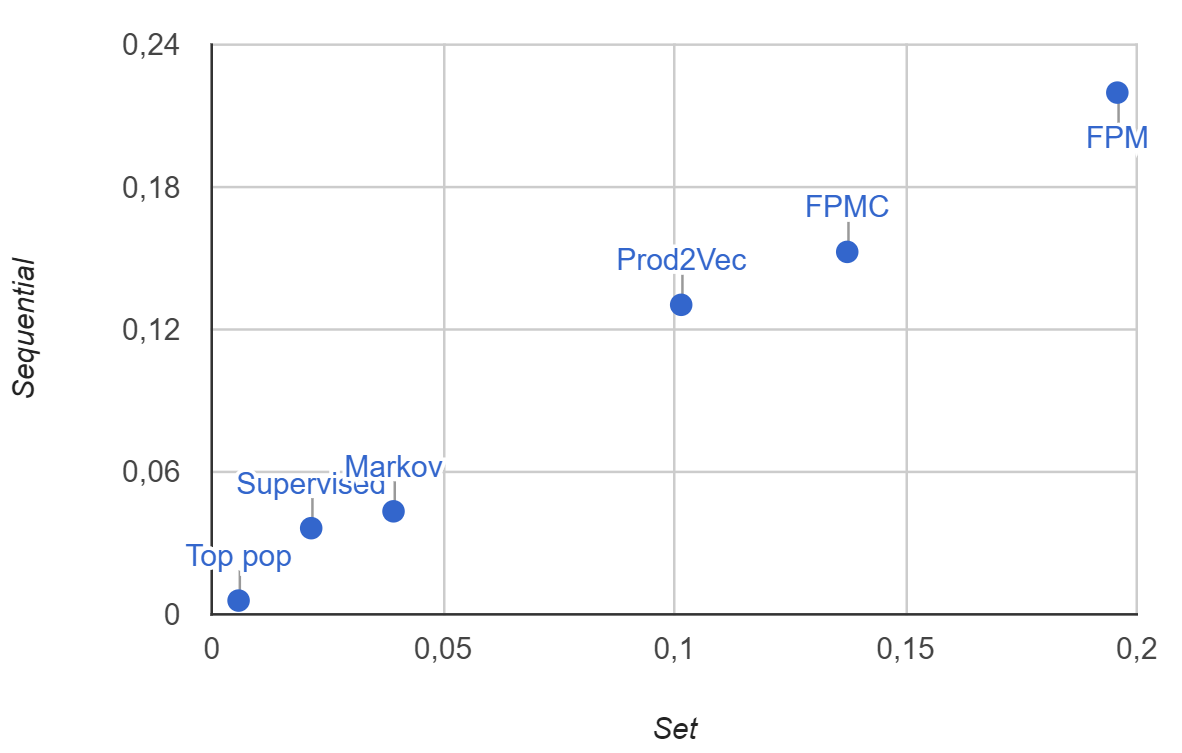
\includegraphics[width=0.8\textwidth]{img/recall_k_1.png}
	\caption{Recall scores for the set evaluation and the sequential evaluation, with $k=1$.}
	\label{img:recall_k_1}
\end{figure}

\begin{figure}[H]
	\centering			
	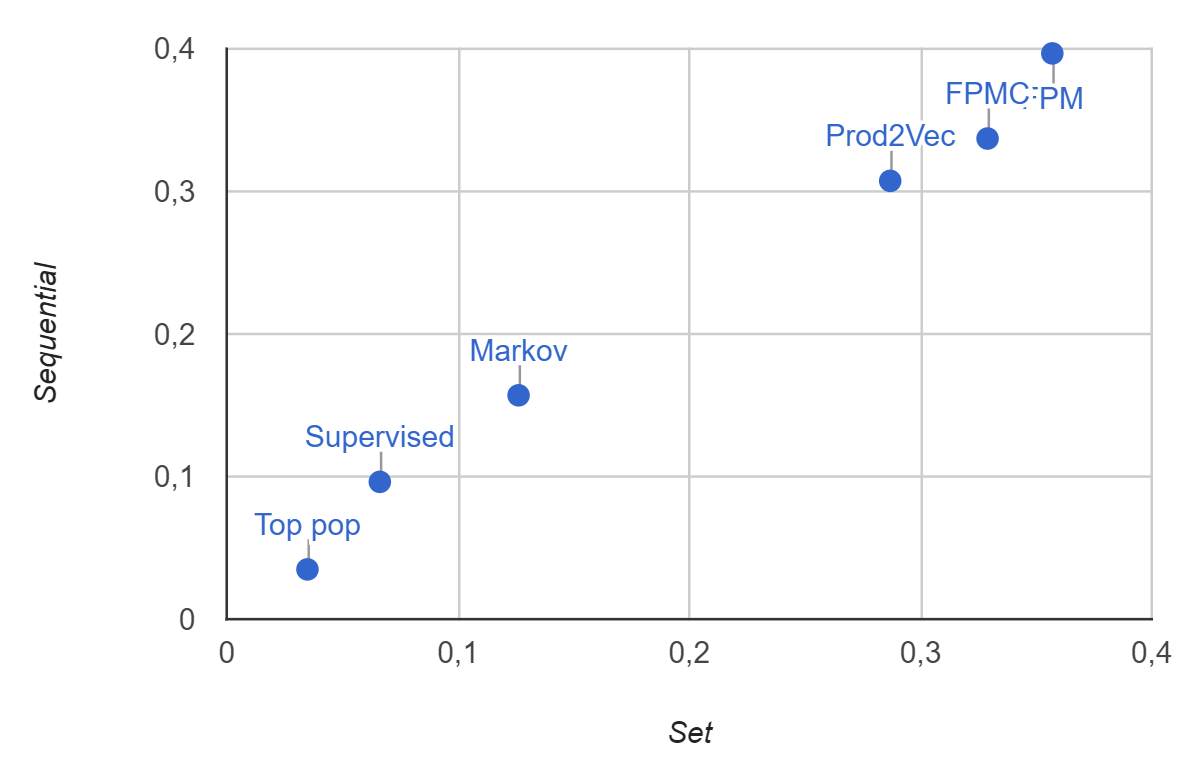
\includegraphics[width=0.8\textwidth]{img/recall_k_5.png}
	\caption{Recall scores for the set evaluation and the sequential evaluation, with $k=5$.}
	\label{img:recall_k_5}
\end{figure}

\begin{figure}[H]
	\centering			
	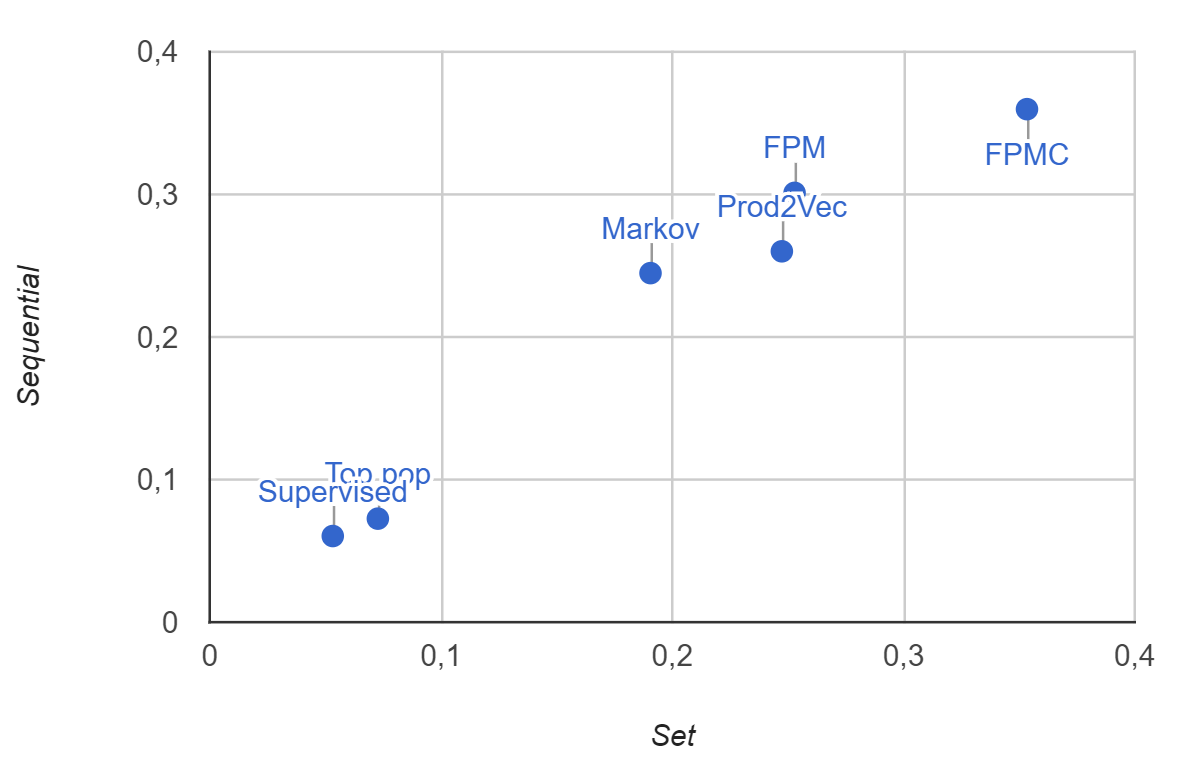
\includegraphics[width=0.8\textwidth]{img/recall_k_10.png}
	\caption{Recall scores for the set evaluation and the sequential evaluation, with $k=10$.}
	\label{img:recall_k_10}
\end{figure}

The sensitivity for the precision score for each $k$ is $(0.9534,  0.9856,  0.618)$ meaning that the set evaluation usually gives much more difference in the evaluation of the recommenders than the sequential one. With respect to the recall instead the sensitivity for each $k$ is $(-0.1463, -0.1227, -0.0994)$ meaning that the magnitude of the scores is almost the same yet slightingly stronger for the sequential evaluation.

\section{SCALING UP}
The analysis done for 500 unique items in the dataset has been extended to 5000 unique items, in so doing the validity of the work is extended to real-world scenarios. The main issue with such a large dataset is that not all the models presented scale to such a large dataset (with the available CPU and memory) or execute in the available amount of time. In order to make the analysis feasible the dataset has been sub-sampled by considering only the last 2 months of interactions (statistics provided in Table~\ref{data5000}).
For each evaluation protocol the recommender have been tested using a profile length of 1, 5, 10 and by calculating the metrics of precision and recall at 5, 10, 100. The results of this analysis are shown in Tables ~\ref{tab:precision5000}~\ref{tab:recall5000}.
The supervised recommender lacks of results is due to the expected execution time ~250h, yet in the few cases in which the execution has terminated the performances were even worst than the top popular recommender.

\begin{table}[H]
	\centering
	\caption{Dataset statistics for 5000 unique items}
	\label{data5000}
	\begin{tabular}{|c|c|c|c|}
		\hline
		\textbf{k} & \textbf{Train Size} & \textbf{Test Size} & \textbf{Average sequence length} \\ \hline
		1          & 92466              & 23117              & 7.39                           \\ \hline
		5          & 44767               & 11192               & 11.64                            \\ \hline
		10         & 17497                & 4375               & 17.98                          \\ \hline
	\end{tabular}
\end{table}


% Table generated by Excel2LaTeX from sheet '5000'
\begin{table}[htbp]
	\centering
	\caption{Precision scores at 5, 10, 100 using two different evaluation protocols: set and sequential. For each protocol results are reported for user profile length of 1, 5, 10. Values in bold are the best score for a particular choice of user profile length and evaluation protocol (Column).}
	\begin{tabular}{|c|c|c|c|c|c|c|c|}
		\cmidrule{3-8}    \multicolumn{1}{c}{} &       & \multicolumn{3}{c|}{Set} & \multicolumn{3}{c|}{Seq} \\
		\cmidrule{3-8}    \multicolumn{1}{c}{} &       & 1     & 5     & 10    & 1     & 5     & 10 \\
		\midrule
		\multirow{3}[6]{*}{FPM} & precision@5 & 0.0844 & 0.2233 & \textbf{0.1998} & 0.0389 & \textbf{0.1094} & \textbf{0.1015} \\
		\cmidrule{2-8}          & precision@10 & 0.0832 & 0.2214 & 0.1977 & 0.0377 & 0.108 & 0.1002 \\
		\cmidrule{2-8}          & precision@100 & 0.0828 & 0.2203 & 0.1969 & 0.0377 & 0.1078 & 0.1001 \\
		\midrule
		\multirow{3}[6]{*}{FPMC} & precision@5 & 0.1747 & 0.1791 & 0.1234 & 0.4213 & 0.0385 & 0.0281 \\
		\cmidrule{2-8}          & precision@10 & 0.1429 & 0.1475 & 0.0956 & 0.031 & 0.0301 & 0.0195 \\
		\cmidrule{2-8}          & precision@100 & 0.0265 & 0.0284 & 0.0213 & 0.0053 & 0.0052 & 0.0036 \\
		\midrule
		\multirow{3}[6]{*}{Supervised} & precision@5 & -     & -     & -     & -     & -     & - \\
		\cmidrule{2-8}          & precision@10 & -     & -     & -     & -     & -     & - \\
		\cmidrule{2-8}          & precision@100 & 0.0024 & -     & -     & -     & -     & - \\
		\midrule
		\multirow{3}[6]{*}{Prod2Vec} & precision@5 & \textbf{0.2112} & 0.\textbf{2504} & 0.185 & \textbf{0.0576} & 0.066 & 0.0503 \\
		\cmidrule{2-8}          & precision@10 & 0.1644 & 0.1766 & 0.129 & 0.0355 & 0.0386 & 0.0293 \\
		\cmidrule{2-8}          & precision@100 & 0.1644 & 0.1766 & 0.129 & 0.0355 & 0.0386 & 0.0293 \\
		\midrule
		\multirow{3}[6]{*}{Popular} & precision@5 & 0.0115 & 0.0119 & 0.0142 & 0.0016 & 0.0018 & 0.0018 \\
		\cmidrule{2-8}          & precision@10 & 0.0105 & 0.0114 & 0.0131 & 0.0014 & 0.0016 & 0,0017 \\
		\cmidrule{2-8}          & precision@100 & 0.0056 & 0.0064 & 0.0072 & 0.0008 & 0.0009 & 0.0009 \\
		\midrule
		\multirow{3}[6]{*}{Markov} & precision@5 & 0.0751 & 0.141 & 0.153 & 0.0328 & 0.0571 & 0.0552 \\
		\cmidrule{2-8}          & precision@10 & 0.0762 & 0.1237 & 0.1216 & 0.0263 & 0.037 & 0.0326 \\
		\cmidrule{2-8}          & precision@100 & 0.0253 & 0.0288 & 0.0315 & 0.0051 & 0.0058 & 0.0059 \\
		\midrule
	\end{tabular}%
	\label{tab:precision5000}%
\end{table}%

% Table generated by Excel2LaTeX from sheet '5000'
\begin{table}[htbp]
	\centering
	\caption{Recall scores at 5, 10, 100 using two different evaluation protocols: set and sequential. For each protocol results are reported for user profile length of 1, 5, 10.Values in bold are the best score for a particular choice of user profile length and evaluation protocol (Column).}
	\begin{tabular}{|c|c|c|c|c|c|c|c|}
\cmidrule{3-8}    \multicolumn{1}{c}{} &       & \multicolumn{3}{c|}{Set} & \multicolumn{3}{c|}{Seq} \\
		\cmidrule{3-8}    \multicolumn{1}{c}{} &       & 1     & 5     & 10    & 1     & 5     & 10 \\
		\midrule
		\multirow{3}[6]{*}{FPM} & recall@5 & 0.0479 & 0.1615 & 0.1403 & 0.0837 & 0.2281 & 0.1967 \\
		\cmidrule{2-8}          & recall@10 & 0.0622 & 0.1872 & 0.1623 & 0.0881 & 0.2459 & 0.2163 \\
		\cmidrule{2-8}          & recall@100 & 0.0658 & 0.1911 & 0.1701 & 0.0892 & 0.2489 & 0.2243 \\
		\midrule
		\multirow{3}[6]{*}{FPMC} & recall@5 & 0.1799 & 0.1853 & 0.1376 & 0.2106 & 0.1927 & 0.1409 \\
		\cmidrule{2-8}          & recall@10 & 0.2667 & 0.2902 & 0.1901 & 0.3109 & 0.3014 & 0.1955 \\
		\cmidrule{2-8}          & recall@100 & \textbf{0.4606} & 0.5027 & 0.3548 & \textbf{0.5344} & 0.5249 & 0.3657 \\
		\midrule
		\multirow{3}[6]{*}{Supervised} & recall@5 & -     & -     & -     & -     & -     & - \\
		\cmidrule{2-8}          & recall@10 & -     & -     & -     & -     & -     & - \\
		\cmidrule{2-8}          & recall@100 & 0.0419 & -     & -     & -     & -     & - \\
		\midrule
		\multirow{3}[6]{*}{Prod2Vec} & recall@5 & 0.2114 & 0.2792 & 0.2184 & 0.2883 & 0.3301 & 0.2516 \\
		\cmidrule{2-8}          & recall@10 & 0.301 & 0.36  & 0.271 & 0.3556 & 0.3866 & 0.2939 \\
		\cmidrule{2-8}          & recall@100 & 0.301 & 0.36  & 0.271 & 0.3556 & 0.3866 & 0.2939 \\
		\midrule
		\multirow{3}[6]{*}{Popular} & recall@5 & 0.0083 & 0.0092 & 0.0089 & 0.0083 & 0.0092 & 0.009 \\
		\cmidrule{2-8}          & recall@10 & 0.0148 & 0.0168 & 0.0168 & 0.0149 & 0.0169 & 0.017 \\
		\cmidrule{2-8}          & recall@100 & 0.0786 & 0.0922 & 0.0915 & 0.079 & 0.0924 & 0.092 \\
		\midrule
		\multirow{3}[6]{*}{Markov} & recall@5 & 0.0829 & 0.1737 & 0.1892 & 0.1643 & 0.2859 & 0.2776 \\
		\cmidrule{2-8}          & recall@10 & 0.1573 & 0.2742 & 0.2602 & 0.2636 & 0.3703 & 0.3269 \\
		\cmidrule{2-8}          & recall@100 & 0.4312 & \textbf{0.5211} & \textbf{0.5171} & 0.5003 & \textbf{0.5674} & \textbf{0.5563} \\
		\midrule
	\end{tabular}%
	\label{tab:recall5000}%
\end{table}%

In order to understand the difference between the two evaluation protocols, for each choice of user profile length and metrics at $n$ the rankings among the recommenders have been calculated and are presented in table ~\ref{tab:rankings}. From this results it can be seen that the ranking for each metric using any protocol in the same, just if few cases some recommenders have slightly different position. As it was proved in with the experiment using only 500 items all the $r$ values are 1 except for few which are 0.8. This analysis strengthen the conclusion that the two evaluation protocols lead to the same ranking thus it can be favorable to adopt the set evaluation which is faster. As regards computation time, all the results of this work have been generated with a CPU i7@2.60GHz with 16GB of RAM, for each recommender the average execution time for set and sequential protocols in the worst case (user-profile length is 1 and the metric@100) is reported in table~\ref{tab:time}.

% Table generated by Excel2LaTeX from sheet '5000'
\begin{table}[htbp]
	\centering
	\caption{Execution times.}
	\begin{tabular}{|c|r|r|r|r|r|}
		\toprule
		& \multicolumn{1}{c|}{FPMC} & \multicolumn{1}{c|}{Markov} & \multicolumn{1}{c|}{FPM} & \multicolumn{1}{c|}{Prov2Vec} & \multicolumn{1}{c|}{Supervised} \\
		\midrule
		Training & 5m    & 6h    & 5m    & 1m    & 1h \\
		\midrule
		Set   & 4h    & 1.5h  & 1h    & 30s   & 14h \\
		\midrule
		Seq   & 23h   & 10h   & 39h   & 2.5m  & $>$ 250h (estimate) \\
		
		\bottomrule
	\end{tabular}%
	\label{tab:time}%
\end{table}%


% Table generated by Excel2LaTeX from sheet '5000'
\begin{table}[ht]
	\centering
	\caption{Rankings given the scores for precision and recall of each recommender. The recommenders are ordered from the best to the worst.}
	\begin{tabular}{|c|l|l|}
		\toprule
		& \multicolumn{1}{c|}{precision@5} & \multicolumn{1}{c|}{recall@5} \\
		\bottomrule
		set  1 & p2v-fpmc-fpm-markov-pop & p2v-fpmc-markov-fpm-pop \\
		\midrule
		seq 1 & p2v-fpmc-fpm-markov-pop & p2v-fpmc-markov-fpm-pop \\
		\midrule
		\midrule
		set 5 & p2v-fpm-markov-fpmc-pop & p2v-fmpc-markov-fpm-pop \\
		\midrule
		seq 5 & fpm-p2v-marvok-fpmc-pop & p2v-markov-fpm-fpmc-pop \\
		\midrule
		\midrule
		set 10 & fpm-p2v-marvok-fpmc-pop & p2v-markov-fpm-fpmc-pop \\
		\midrule
		seq 10 & fpm-markov-p2v-fpmc-pop & markov-p2v-fpm-fpmc-pop \\
	\toprule
		\multicolumn{1}{r|}{} & \multicolumn{1}{c|}{precision@10} & \multicolumn{1}{c|}{recall@10} \\
			\bottomrule
		set  1 & p2v-fpmc-fpm-markov-pop & p2v-fpmc-markov-fpm-pop \\
		\midrule
		seq 1 & fpm-p2v-fpmc-markov-pop & p2v-fpmc-markov-fpm-pop \\
		\midrule
		\midrule
		set 5 & fpm-p2v-fpmc-markov-pop & p2v-fpmc-markov-pfm-pop \\
		\midrule
		seq 5 & fpm-p2v-fpmc-markov-pop & p2v-markov-fpmc-fpm-pop \\
		\midrule
		\midrule
		set 10 & fpm-p2v-markov-fpmc-pop & p2v-markov-fpmc-fpm-pop \\
		\midrule
		seq 10 & fpm-markov-p2v-fpmc-pop & markov-p2v-fpm-fpmc-pop \\
		\toprule
		\multicolumn{1}{r|}{} & \multicolumn{1}{c|}{precision@100} & \multicolumn{1}{c|}{recall@100} \\
		\bottomrule
		set  1 & p2v-fpm-fpmc-markov-pop-supervised & fpmc-markov-p2v-fpm-pop-supervised \\
		\midrule
		seq 1 & fpm-p2v-fpmc-markov-pop & fpmc-markov-p2v-fpm-pop \\
		\midrule
		\midrule
		set 5 & fpm-p2v-markov-fpmc-pop & markov-fpmc-p2v-fpm-pop \\
		\midrule
		seq 5 & fpm-p2v-markov-fpmc-pop & markov-fpmc-p2v-fpm-pop \\
		\midrule
		\midrule
		set 10 & fpm-p2v-markov-fpmc-pop & markov-fpmc-p2v-fpm-pop \\
		\midrule
		seq 10 & fpm-p2v-markov-fpmc-pop & markov-fpmc-p2v-fpm-pop \\
		\bottomrule
	\end{tabular}%
	\label{tab:rankings}%
\end{table}%



\section{CONCLUSION}
In this work two evaluation protocols (i.e. set and sequential) for SRS are compared with respect to the ranking produced among the recommenders using both precision and recall. Six classes of state-of-the-art SRS are implemented in order to perform such evaluation. The analysis takes into account several values of $k$ (i.e. length of user profile) and assesses the difference among the two evaluation protocols in terms of $r$ value and sensitivity. By analyzing the $r$ value it is possible to conclude that the rankings produced by the two protocols are the same except for one case where the $r$ value is a little lower than 1. The analysis using the sensitivity value highlights the fact that the precision metric calculated using the set protocol usually gives much bigger gaps between the SRS whilst for the recall is close to 0. The conclusion that can be drawn from this work is that when one has to choose between the two protocols, and the use of the recommender (i.e. application scope) does not enforce one choice over the other, the set evaluation is advised because it gives a clearer picture of the difference among recommenders performance, moreover it is much faster to evaluate than the sequential one.




\newpage
\section{APPENDIX}
\subsection{}
The code repo is available at :\href{https://umbertoDifa@bitbucket.org/umbertoDifa/seq_rec_evaluation.git}{https://umbertoDifa@bitbucket.org/umbertoDifa/seq\_rec\_evaluation.git}
\subsection{}
\begin{itemize}
	\item \textbf{Popularity}
		\begin{description}
		\item [Top n = 5] Number of items recommended.
	\end{description}
	\item \textbf{Frequent Pattern Mining}: 
		\begin{description}
			\item [Min context = 1] The minimum context used while applying the all-kth algorithm\cite{nakagawa03impact}.
			\item [Max context = 10] The maximum context for the all-kth algorithm.
			\item [Min support = 0.002] Minimum support for frequent sequence mining.
			\item [Min confidence = 0.1] Minimum confidence to recommend an item.
						\item [Top n = 5] Number of items recommended.
		\end{description}
	\item \textbf{Markov Chain}
		\begin{description}
				\item [From k = 1] Minimum order or the model.
				\item [To k = 11] Maximum order of the model.
							\item [Top n = 5] Number of items recommended.
		\end{description}
	\item \textbf{Prod2Vec} 
	\begin{description}
		\item [Min count = 10] Minimum occurrences of an item, in order to be considered.
		\item [Size = 300]  The dimensionality of the feature vectors..
		\item [Window = 5]  The maximum distance between the current and predicted item within a sequence.
		\item [Top n = 5] Number of items recommended.
	\end{description}
	\item \textbf{Supervised} 
	\begin{description}
		\item [History length = 1] Length of history to consider acconrding to the data expansion model.\cite{zidmars01temporal}
					\item [Top n = 5] Number of items recommended.
	\end{description}
	\item \textbf{Factorizing Personalized Markov Chains} 
		\begin{description}
			\item [Latent factors = 92] Number of latent factors.
			\item [Learning rate = 0.01] Learning rate
			\item [Regularization = 0.001] Regularization term
			\item [Epochs = 40] Number of epochs		
			\item [Negative samples = 10] Number of negative samples			
			\item [Top n = 5] Number of items recommended.
	\end{description}
\end{itemize}
%struttura progetto, scalabilita'
%comandi principali


%%%%%%%%%%%%%%%%%%%%%%%%%%%%%%%%%%%%%%%%%%%%%%%%%%%%%%%%%%%%%%%%%%%%%%%%%%%%%%%%


\bibliographystyle{ACM-Reference-Format-Journals}
\bibliography{bibliography}

\end{document}

